% Derived from the completed Thesis_Chapter.qmd, 2026-10-02.
% Numeric sources and exhibit fates: docs/plans/manuscript_completion_findings_2026-10-02.md.
% CTJ_Reading.tex selects the reading layout; this file defaults to submission.
\newif\ifctjreading
\ifdefined\CTJReadingVersion
  \ctjreadingtrue
  \documentclass[Afour,sagev,times]{sagej}
\else
  \ctjreadingfalse
  \documentclass[Review,sagev,times,doublespace,12pt]{sagej}
\fi
\usepackage{amsmath,booktabs,graphicx,array}
\usepackage{url}
% Yellow highlight for placeholder text that must be finalized before submission.
\usepackage{xcolor,soul}
\sethlcolor{yellow}
\ifctjreading
  % Balance only the final reading page's columns (balance's \balance also
  % evened earlier pages, pushing References to a new page).
  \usepackage{flushend}
  \geometry{headheight=20pt}
  \setlength{\emergencystretch}{2em}
  \raggedbottom
\else
  \usepackage{lastpage}
  \geometry{a4paper,margin=25mm,headheight=20pt}
\fi
\ifctjreading
  \usepackage[hidelinks,bookmarksopen,bookmarksnumbered]{hyperref}
\else
  \usepackage[colorlinks,bookmarksopen,bookmarksnumbered,citecolor=blue,urlcolor=blue]{hyperref}
\fi
\usepackage[switch]{lineno}
\renewcommand\linenumberfont{\normalfont\tiny\sffamily}
\setlength\linenumbersep{3pt}
\def\volumeyear{2026}
\def\journalname{Clinical Trials}
\def\volumenumber{Submission draft\ }
\def\issuenumber{review}
% One source owns the title, abstract, authors, body and all exhibit content.
\newcommand{\CTJTitle}{Sampling Design for Spatial Cluster Randomized Trials Under Heterogeneous Incidence}
\newcommand{\CTJAuthorLine}{Andrew Walther\textsuperscript{1}, Ashkan Habib\textsuperscript{2}, Ross Joseph Simpson, Jr.\textsuperscript{3}, and Feng-Chang Lin\textsuperscript{1}}
\newcommand{\CTJAffilOne}{\textsuperscript{1}Department of Biostatistics, University of North Carolina at Chapel Hill, Chapel Hill, NC, USA}
\newcommand{\CTJAffilTwo}{\textsuperscript{2}Department of Epidemiology, University of North Carolina at Chapel Hill, Chapel Hill, NC, USA}
\newcommand{\CTJAffilThree}{\textsuperscript{3}Division of Cardiology, University of North Carolina School of Medicine, Chapel Hill, NC, USA}
\newcommand{\CTJContact}{Feng-Chang Lin, Department of Biostatistics, University of North Carolina at Chapel Hill, Chapel Hill, NC 27599, USA.}
\newcommand{\CTJKeywords}{cluster randomized trial; spatial spillover; interference; design-stage treatment allocation; incidence-guided design; sudden unexpected death}
\newcommand{\CTJAbstract}{%
\textbf{Background/Aims:} In spatial cluster randomized trials, treatment effects can spill over and contaminate clusters that neighbor treated clusters, so the choice of which clusters to treat affects how accurately the treatment effect can be estimated. We compared six treatment assignment designs and simple random sampling (SRS) on two criteria, the average estimation error and the error under an unfavorable realized assignment (allocation risk). We then applied the designs to planning a sudden unexpected death (SUD) prevention education pilot in North Carolina.

\textbf{Methods:} We simulated trials on a $10\times10$ grid of 100 clusters, varying incidence heterogeneity, spatial dependence, spillover magnitude, spillover regime (effects reaching only untreated neighbors, or neighbors in both arms) and treatment-effect size. The treatment effect was estimated with a maximum likelihood spatial autoregressive (spatial lag) model, and accuracy was measured by mean squared error (MSE). The application used observed 2018--2021 SUD incidence in 58 North Carolina community-college service-area clusters to decide which clusters were treated, and it simulated a continuous education outcome that does not depend on incidence. Neighbors were defined by queen contiguity in the primary analysis. Sensitivity analyses used rook contiguity, added an incidence-related baseline to the outcome, and ordered regions by alternative incidence summaries.

\textbf{Results:} The spillover regime determined which designs performed best. On the grid with treatment effect $\tau=1$, Incidence-Guided Saturation had a control-only mean MSE of 0.1355, compared with 0.2146 for SRS, while under both-arms spillover no design was detectably more accurate than SRS. In the North Carolina application, Incidence-Guided Saturation lowered control-only mean MSE by 21.1--29.9\% relative to SRS, depending on the year, and its worst-performing assignments also had lower error than those of SRS. Under both-arms spillover, SRS and several randomized designs had similar accuracy. Across application designs, 95\% $t$-based confidence intervals with a degrees-of-freedom correction covered the true effect 94.2--94.9\% of the time, compared with 92.7--93.6\% for standard Wald intervals.

\textbf{Conclusions:} When spillover is expected mainly in control clusters, Incidence-Guided Saturation, which treats larger shares of clusters in higher-incidence regions, had the lowest or near-lowest estimation error and lower allocation risk than SRS, while giving the highest-burden region the largest treated share. When spillover reaches both arms, SRS remains competitive. Design choice should also weigh model assumptions, the number of clusters treated and the share of the population they contain, and whether enough clusters are available for adequate power. This study evaluates trial designs, not the effectiveness of an implemented intervention.
}
% Shared approved exhibit definitions for both CTJ layouts.
% Author: Andrew Walther. Updated: 2026-10-27.
% Figure sources: code/20_manuscript_figure_revision.R; no simulation rerun.
% Table 1 example maps: code/25_design_assignment_figures.R (illustrative surface).
% Starred floats span both reading columns; every macro is called once per build.

% One example map per Table 1 row, vertically centered with padding between rows;
% \CTJCat sets each design's category on an italic line under its name.
\newcommand{\CTJCat}[1]{\newline{\footnotesize\textit{#1}}}
\newcommand{\CTJThumb}[1]{\raisebox{-0.5\height}{\includegraphics[width=1.9cm]{../figures/compact/design_thumbs/thumb_#1.pdf}}\rule[-1.05cm]{0pt}{2.2cm}}
\newcommand{\CTJDesignTable}{%
\begin{table*}[!htb]
\small
\centering
\caption{Treatment assignment designs on the 100-cluster grid and their North Carolina (NC) adaptations, each with its category (italic) and one example assignment on the grid (blue, treated; white, control). Every example uses the incidence surface in the first row, a representative spatial surface (incidence dependence $\rho_X=0.5$) drawn for illustration. Numbers in the Balanced Quartiles example give each cluster's incidence quartile; percentages in the Incidence-Guided Saturation example give each quadrant's treated share. Incidence is the simulated grid covariate or the observed annual cluster rate. Two related variants, Saturation Quadrants (randomly ordered quadrants) and Balanced Halves (balancing within incidence halves), performed similarly to their retained counterparts and are reported in the supplementary information (SI).}
\label{tab:allocation-rules}
\begin{tabular}{>{\raggedright\arraybackslash}m{0.16\linewidth}c>{\raggedright\arraybackslash}m{0.35\linewidth}>{\raggedright\arraybackslash}m{0.27\linewidth}}
\toprule
Design & Example (grid) & Grid (100 clusters) & NC (58 clusters) \\
\midrule
\textit{Incidence surface} & \CTJThumb{incidence} & Representative incidence surface used in the design examples below; darker cells represent higher incidence, and dashed lines mark quadrant boundaries. & Observed annual SUD rate of each cluster. \\
Checkerboard\CTJCat{Fixed spatial interspersion} & \CTJThumb{1} & Treat alternating clusters in a checkerboard pattern, so no two clusters that share an edge are in the same arm (50 treated). & Deterministic map version that visits clusters from most to fewest neighbors and gives each the arm less common among its assigned neighbors (27 treated). \\
High Incidence Focus\CTJCat{Incidence targeting} & \CTJThumb{2} & Treat the 50 clusters with the highest incidence, with ties broken at random (50 treated). & Treat the clusters with the highest observed rate (29 treated). \\
Isolation Buffer\CTJCat{Spatial separation} & \CTJThumb{4} & Treat clusters one at a time, each chosen at random from the untreated clusters with no treated neighbor, until none remain, so no two treated clusters are neighbors (about 21 treated with queen neighbors). & Same rule on the NC adjacency graph (about 16 treated). \\
$2\times2$ Blocking\CTJCat{Local spatial balance} & \CTJThumb{5} & Divide the grid into 25 blocks of $2\times2$ clusters and treat two randomly chosen clusters in each block (50 treated). & Spatial blocking, which treats a random half (rounded) of each of 14 groups formed each year by $k$-means clustering on location, incidence rank and log-population (27--31 treated by year). \\
Balanced Quartiles\CTJCat{Incidence balance} & \CTJThumb{6} & Divide clusters into quartiles of incidence rank and randomly treat half of the clusters in each quartile (50 treated). & Same rule with observed rates (29 treated). \\
Incidence-Guided Saturation\CTJCat{Incidence-ordered regional saturation} & \CTJThumb{8} & Treat a random 80\%, 60\%, 40\% and 20\% of the clusters in the four $5\times5$ quadrants, ordered from highest to lowest mean incidence (50 treated). & Same rule with four fixed geographic regions, ordered by the mean rank of their clusters' observed rates (29 treated). \\
Simple Random Sampling\CTJCat{Unrestricted reference} & \CTJThumb{9} & Treat a completely random half of the clusters (50 treated). & Same rule (29 treated). \\
\bottomrule
\end{tabular}
\end{table*}
}

\newcommand{\CTJGridTable}{%
\begin{table*}[!htb]
\small
\centering
\caption{Grid benchmark at $\tau=1$ with queen contiguity. Each regime-specific entry averages 80 scenarios (five incidence configurations, four outcome-dependence values $\rho$ and four spillover-magnitude values $\gamma$). MSE is the mean squared error of the estimate of $\tau$, and coverage is the proportion of 95\% $t$-based confidence intervals (CIs), with a degrees-of-freedom-corrected standard error, that contain $\tau$. Both use the spatial lag model that includes the true spillover term. The ratio to SRS divides each design's MSE by that of simple random sampling (SRS), which randomly selects 50 of the 100 clusters for treatment. Its 95\% interval is one plus the paired design-minus-SRS interval for the mean difference in MSE across the 50 independent configuration-by-surface units, divided by the SRS MSE, so an interval excluding 1 indicates a difference larger than simulation error (no adjustment for multiple comparisons).}
\label{tab:grid-srs}
% SOURCE: results/srs_benchmark/manuscript_regime_means.csv (MSE, coverage);
% results/srs_benchmark/manuscript_paired_ratios.csv (ratios; code/19 from code/15).
\setlength{\tabcolsep}{4pt}
\begin{tabular}{lrrcrrc}
\toprule
& \multicolumn{3}{c}{Both arms} & \multicolumn{3}{c}{Control only} \\
\cmidrule(lr){2-4}\cmidrule(lr){5-7}
Design & MSE & Coverage & Ratio to SRS (95\% CI) & MSE & Coverage & Ratio to SRS (95\% CI) \\
\midrule
Checkerboard & 0.0624 & 0.948 & 1.47 (1.44, 1.51) & 2.1114 & 0.951 & 9.84 (9.65, 10.03) \\
High Incidence Focus & 0.1617 & 0.950 & 3.82 (3.71, 3.92) & 0.3292 & 0.945 & 1.53 (1.45, 1.62) \\
Isolation Buffer & 0.1608 & 0.948 & 3.80 (3.72, 3.87) & 0.1595 & 0.950 & 0.74 (0.72, 0.77) \\
$2\times2$ Blocking & 0.0623 & 0.947 & 1.47 (1.44, 1.50) & 0.5761 & 0.950 & 2.68 (2.62, 2.74) \\
Balanced Quartiles & 0.0421 & 0.949 & 0.99 (0.97, 1.02) & 0.2195 & 0.942 & 1.02 (1.00, 1.05) \\
Incidence-Guided Saturation & 0.0459 & 0.949 & 1.08 (1.06, 1.11) & 0.1355 & 0.945 & 0.63 (0.61, 0.65) \\
Simple Random Sampling & 0.0424 & 0.950 & N/A & 0.2146 & 0.946 & N/A \\
\bottomrule
\end{tabular}
\end{table*}
}

\newcommand{\CTJMapFigure}{%
\begin{figure*}[tp]
\centering
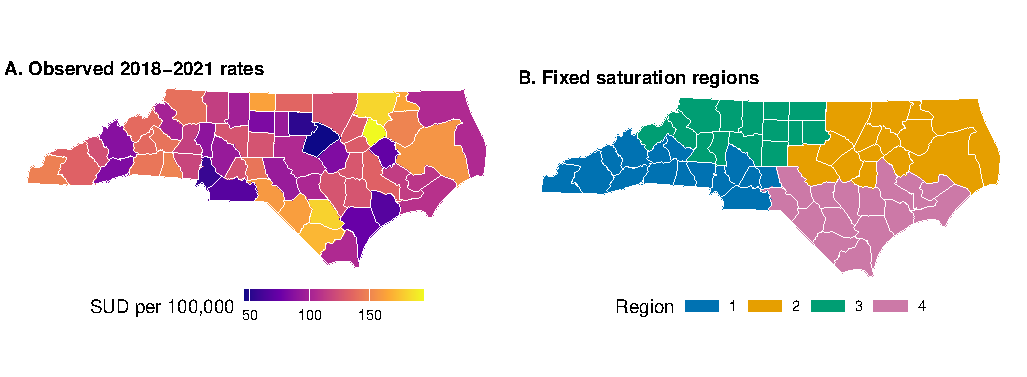
\includegraphics[width=\linewidth]{../figures/compact/nc_planning_map.pdf}
\caption{Observed North Carolina sudden unexpected death (SUD) incidence. (A) SUD rates per 100,000 population aged 18--64 for the 58 service-area clusters, pooled over 2018--2021 (deaths divided by person-years). (B) The fixed four-region partition used by Incidence-Guided Saturation in every year. (C) Annual rates on the same color scale. Each year is analyzed separately, so the year-to-year shifts in panel C explain why some designs' results vary by year (Figure~\ref{fig:nc-mse}). Incidence guides treatment allocation only and does not enter the education outcome.}\label{fig:nc-map}
\end{figure*}
}

\newcommand{\CTJGridFigure}{%
\begin{figure*}[tp]
\centering
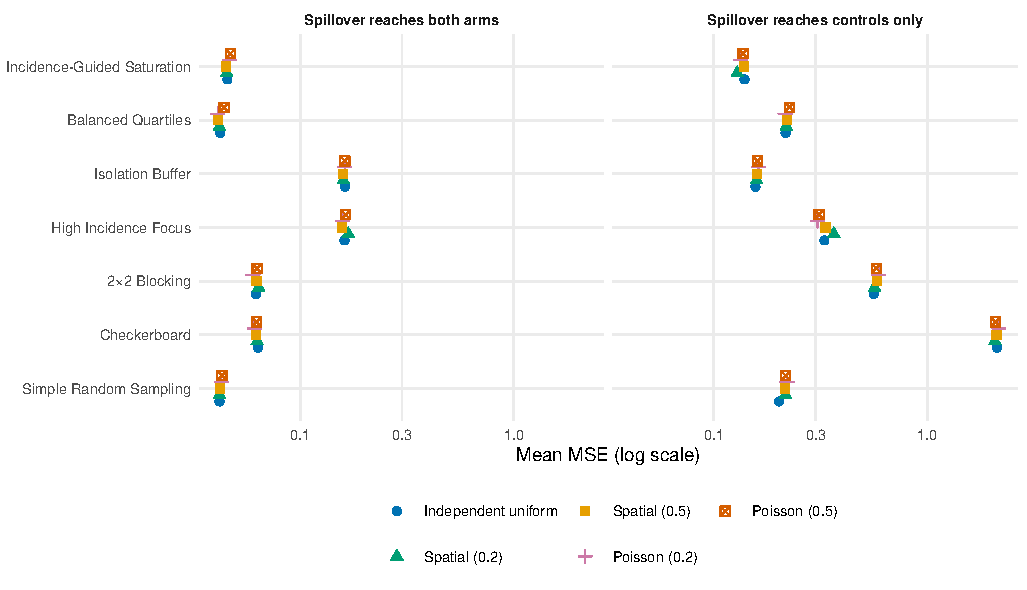
\includegraphics[width=\linewidth]{../figures/compact/grid_accuracy_srs.pdf}
\caption{Grid mean MSE at $\tau=1$ with queen contiguity for the six designs and simple random sampling. Results are shown separately for the five incidence configurations, each averaging the 16 outcome-dependence and spillover-magnitude settings within its spillover regime. Parentheses in the legend give the incidence dependence $\rho_X$. Incidence configuration changes mean MSE little for every design except High Incidence Focus. Horizontal lines are 95\% Monte Carlo intervals over the ten simulated incidence surfaces and are often narrower than the symbols. Designs share surfaces and outcome noise, so Table~\ref{tab:grid-srs} gives the paired comparison of each design with simple random sampling.}\label{fig:grid}
\end{figure*}
}

\newcommand{\CTJAllocationFigure}{%
\begin{figure*}[tp]
\centering
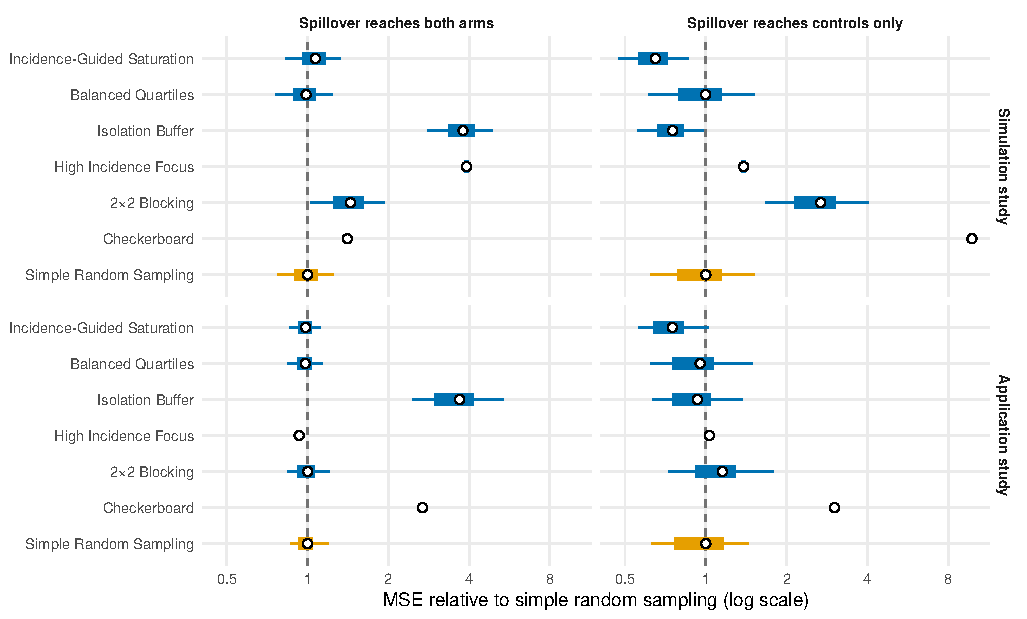
\includegraphics[width=\linewidth]{../figures/compact/allocation_distribution_by_design.pdf}
\caption{Distribution of assignment-specific MSE for the six designs and simple random sampling (SRS), relative to the mean MSE of SRS in the same setting (queen contiguity, $\tau=1$). Figure~\ref{fig:grid} and Table~\ref{tab:grid-srs} report average MSE, whereas this figure shows how MSE varies from one assignment to another (allocation risk). Grid results use all 50 configuration-by-surface units at $\rho\in\{0,0.5\}$ and $\gamma\in\{0.5,0.8\}$, and application results use $\rho\in\{0,0.5\}$ and $\gamma=0.8$ in each year 2018--2021. In the application, $2\times2$ Blocking denotes its spatial-blocking adaptation. Thin lines span the 5th to 95th percentiles of assignments, thick bars the 25th to 75th, and circles mark the mean ratio. Percentiles and means are computed within each setting and then averaged across settings. Outcome noise from the finite number of outcomes per assignment widens the bars, and worst-decile means are reported in the text. A design with one possible assignment per setting appears as a circle only.}\label{fig:alloc-dist}
\end{figure*}
}

\newcommand{\CTJMeanFigure}{%
\begin{figure*}[tp]
\centering
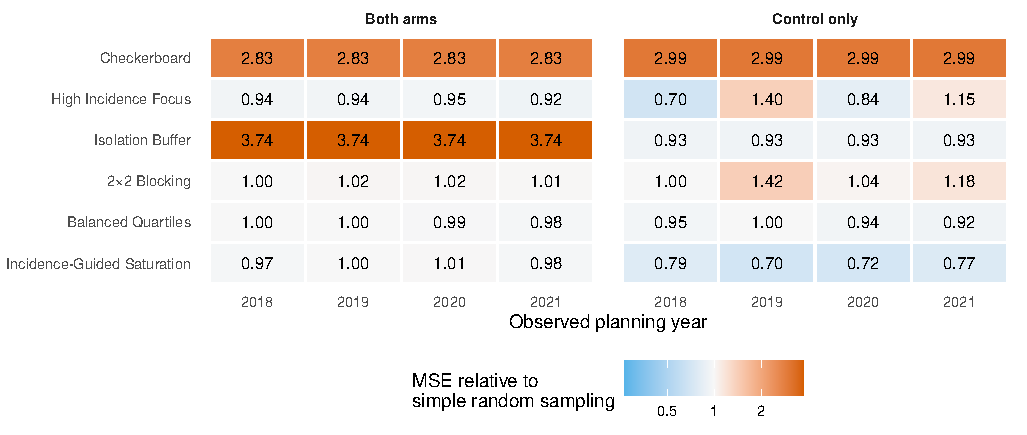
\includegraphics[width=\linewidth]{../figures/compact/nc_annual_accuracy_six.pdf}
\caption{Application mean MSE by year, divided by the mean MSE of simple random sampling (SRS) in the same year and spillover regime, for the six designs with queen contiguity. Each cell averages six $\rho$ and $\gamma$ settings. Blue indicates lower error than SRS and orange higher error, on a logarithmic color scale. SRS mean MSE is 0.07638 under both arms and 0.30761 under control-only spillover. In the application, $2\times2$ Blocking denotes its spatial-blocking adaptation. Absolute MSE, bias and coverage are in the SI.}\label{fig:nc-mse}
\end{figure*}
}

\ifctjreading
% The class's production title would print an invented DOI/volume. This local
% preview header avoids those fields without modifying the supplied Sage class.
\makeatletter
\def\ps@sagepage{%
  \def\@oddhead{\parbox{\textwidth}{\sffamily\small
    Two-column reading preview\hfill\thepage\\[-4pt]\rule{\textwidth}{0.25pt}}}%
  \let\@evenhead\@oddhead
  \def\@oddfoot{\parbox{\textwidth}{\scriptsize\itshape
    Author reading preview; not publisher proofs.}}%
  \let\@evenfoot\@oddfoot}
\makeatother
\fi
\begin{document}
\ifctjreading
\pagestyle{sagepage}
\twocolumn[{%
\begin{@twocolumnfalse}
\begin{minipage}{\textwidth}
\raggedright
{\sffamily\titlesize\bfseries\CTJTitle\par}
\medskip
{\sffamily\bfseries\CTJAuthorLine\par}
\smallskip
{\footnotesize\CTJAffilOne\par\CTJAffilTwo\par\CTJAffilThree\par
\textbf{Correspondence:} \CTJContact{} Email: \url{flin33@email.unc.edu}.\par}
\medskip
{\small\sffamily\textbf{Abstract}\par\CTJAbstract\par
\medskip\textbf{Keywords:} \CTJKeywords\par}
\medskip
{\footnotesize\itshape Reading preview only. Final author approval remains pending.\par}
\medskip
\end{minipage}
\end{@twocolumnfalse}}]
\label{FirstPage}
\else
\onecolumn
\doublespacing
\raggedright
\hyphenpenalty=10000
\exhyphenpenalty=10000
\linenumbers
\runninghead{Sampling design for spatial CRTs}
% A breakable abstract and separate author title page avoid the class's
% boxed production-layout abstract, which cannot span a review page.
\renewenvironment{abstract}{\section*{Abstract}}{}
\begin{titlepage}
\singlespacing
{\Large\bfseries\CTJTitle\par}
\vspace{15mm}
\CTJAuthorLine
\vspace{8mm}

\CTJAffilOne

\CTJAffilTwo

\CTJAffilThree
\vspace{8mm}

Corresponding author: \CTJContact

Email: \url{flin33@email.unc.edu}

Telephone: (919) 966-9431

ORCID: Andrew Walther, 0000-0002-1932-9653; Feng-Chang Lin, 0000-0002-2638-1775
\vspace{8mm}

Running head: Sampling design for spatial CRTs

Main-text word count: 3,498. Abstract word count: 404.
\vfill
Clinical Trials submission draft. Final submission approval remains pending.
\end{titlepage}
\doublespacing
\begin{abstract}
\CTJAbstract
\end{abstract}
\par\medskip\noindent\textbf{Keywords:} \CTJKeywords\clearpage
\fi

\section{Introduction}
Cluster randomized trials assign groups rather than individuals when interventions operate through clinics, schools or geographic areas.\cite{donner_design_2000,hayes_cluster_2017} Spatial interference challenges the assumption that a cluster's outcome depends only on its own treatment. In practice, adjacent populations can share services, information or environmental exposures, so treating one cluster can change outcomes in its neighbors.\cite{hudgens_toward_2008,jarvis_spatial_2017} Two allocations with the same number of treated clusters can then provide very different information about the treatment effect.

Design-stage methods include covariate-constrained randomization, randomized saturation and independent-set or spatial cluster designs,\cite{crisp_covariate-constrained_2023,baird_optimal_2018,cai_independentset_2023,leung_rateoptimal_2022} which serve different objectives. Balancing measured incidence does not ensure that the effect of treatment can be separated from the effect of treated neighbors, and fully alternating treatment can make the two inseparable. In a strict checkerboard with edge neighbors, for example, a cluster's exposure to treated neighbors is fully determined by its own treatment.

In previous work on small grids, we compared simple random sampling with block stratified sampling, an alternating allocation in which no two clusters that share an edge are in the same arm.\cite{walther_spatialcrt_2026} That work weighed average estimation accuracy against the risk of a poor realized allocation. We extend the question to heterogeneous incidence, a larger study region, additional strategies, and an irregular observed geography. The comparison includes simple random sampling (SRS), meaning complete randomization of a fixed number of clusters, and the alternating allocation, here called Checkerboard. We evaluate both the mean squared error (MSE) of the treatment-effect estimate and how that error varies across possible assignments, without comparing numerical results between the two studies.

Our application supports planning an education intervention for healthcare professionals involved in sudden unexpected death (SUD) prevention. Historical incidence can identify areas of need without implying that education outcomes depend on incidence, so we separate incidence-guided allocation from the simulated education outcome. Incidence can direct resources toward areas of greater historical burden, balance that burden between arms, or vary the share of clusters treated in each region (saturation). None of these goals ensures that treatment can be separated from neighboring exposure. A trial realizes only one assignment, so we evaluated both the average accuracy of each strategy and whether the design with the lowest average error also protects against an unfavorable allocation.

\section{Methods}
\subsection{Outcome model, estimation and allocation risk}
Clusters are linked by a spatial weights matrix $W$. Under queen contiguity two clusters are neighbors when they share an edge or a corner, and under rook contiguity when they share an edge.\cite{bivand_applied_2008} Queen contiguity was used for the primary analysis and rook contiguity for a sensitivity analysis. Each row of $W$ sums to one, so for a treatment indicator vector $Z$, the $i$th element of $WZ$ is the proportion of cluster $i$'s neighbors that are treated. Outcomes followed the spatial autoregressive (SAR) lag model\cite{ord_estimation_1975}
\begin{equation}
\ifctjreading
\begin{aligned}
Y&=(I-\rho W)^{-1}[\tau Z+S(Z)+\beta X+\epsilon],\\
\epsilon&\sim N(0,I),
\end{aligned}
\else
Y=(I-\rho W)^{-1}[\tau Z+S(Z)+\beta X+\epsilon],\qquad \epsilon\sim N(0,I),
\fi
\label{eq:grid}
\end{equation}
where $Y$ is the vector of cluster outcomes, $X$ is cluster incidence, $I$ is the identity matrix, $\epsilon$ is independent standard normal noise (so $\tau$ is in units of its standard deviation) and $\rho$ is the spatial dependence of the outcomes. The direct treatment effect $\tau$ is the effect of a cluster's own treatment before outcomes spread between neighbors through $(I-\rho W)^{-1}$, rather than a total effect. Spillover $S(Z)$ followed one of two regimes, $S(Z)=\gamma WZ$ when exposure reaches clusters in both arms and $S(Z)=\gamma(1-Z)\circ WZ$ when it reaches control clusters only, where $\gamma$ is the spillover magnitude and $\circ$ is the elementwise product. Control-only spillover is classical contamination, in which untreated clusters benefit from treated neighbors, whereas under both-arms spillover treated clusters also gain from treated neighbors. The coefficient $\beta$ sets how strongly incidence shifts the baseline outcome. We set $\beta=1$ in the grid study so that incidence is prognostic, the harder case for designs that use incidence, because treatment can then line up with baseline risk. Investigators can choose $\beta$ to suit their own outcome.

We estimated $\tau$, giving $\hat\tau$, by maximum likelihood (ML), fitting the SAR lag model with an intercept, treatment, the true regime-specific spillover covariate and, in the grid study, incidence.\cite{bivand_comparing_2015} Our own ML routine reproduced the estimates of the \texttt{lagsarlm} function in the R package \texttt{spatialreg} to within $10^{-6}$. This fit assumes that the analyst knows the form of spillover, so a grid sensitivity analysis refit the model without the spillover term. Confidence intervals were $\hat\tau\pm t_{0.975,\,N-p}\,\widehat{\mathrm{SE}}\sqrt{N/(N-p)}$, a $t$-based interval with a degrees-of-freedom-corrected standard error, where $\widehat{\mathrm{SE}}$ is the estimated standard error, $N$ the number of clusters and $p$ the number of estimated coefficients including $\rho$. This interval covered $\tau$ more reliably than the standard Wald interval, $\hat\tau\pm1.96\,\widehat{\mathrm{SE}}$. Accuracy was measured by MSE, the average of $(\hat\tau-\tau)^2$ over simulated trials, and coverage by the proportion of 95\% intervals containing $\tau$.

With rook contiguity, Checkerboard gives $WZ=1-Z$, so treatment and spillover cannot be separated, $\tau$ is not identified (cannot be estimated), and the treatment coefficient estimates $\tau-\gamma$. With queen contiguity, Checkerboard is identified but can be imprecise. Every interior cluster has exactly half its neighbors treated, so under control-only spillover the spillover covariate is a linear function of treatment except at the grid boundary.

A trial realizes one assignment, so we also measured how error varies from assignment to assignment. For an assignment $a$ and fixed incidence $X$, the assignment-specific MSE $m(a)=E_\epsilon[(\hat\tau-\tau)^2\mid a,X]$ is the MSE expected over repeated draws of the outcome noise $\epsilon$ with the assignment held fixed. A design's MSE is the expectation of $m(a)$ over the design's assignment distribution. Across a design's sampled assignments, we summarized allocation risk, the upper tail of $m(a)$, by the mean of the worst 10\% of assignments (worst-decile mean). Outcome noise alone can make one trial's error large even when the assignment's expected MSE is modest, so we estimated each $m(a)$ by averaging squared errors over many simulated outcomes before ranking assignments. A design with only one possible assignment has no spread, although its error can still be high.

\subsection{Treatment assignment designs}
Table~\ref{tab:allocation-rules} describes the six designs and SRS, shows an example assignment of each on the grid and summarizes its adaptation to the application, and the supplementary information (SI) gives full specifications. SRS randomly selects 50 of the 100 clusters for treatment, and on the grid every design treated 50 clusters except Isolation Buffer, whose number treated depended on the neighbor graph. Checkerboard was the only deterministic design. In the designs that rank incidence, ties were broken at random for each assignment, so High Incidence Focus had a single possible assignment unless a tie affected the selection.
\ifctjreading
\CTJDesignTable
\fi

The designs differ in how they handle incidence and spatial exposure. Balanced Quartiles spreads treatment evenly across ranked incidence groups, whereas High Incidence Focus aligns treatment with incidence. $2\times2$ Blocking imposes the same local proportion of treated clusters everywhere, while saturation deliberately varies that proportion between regions. Isolation Buffer prevents treated neighbors, and Checkerboard imposes strong interspersion. These restrictions change how closely a cluster's treatment tracks its share of treated neighbors.

\subsection{Simulation study}
The simulated study region was a $10\times10$ grid of 100 clusters. The simulation crossed $\rho=0,0.01,0.2,0.5$, $\gamma=0.5,0.6,0.7,0.8$, both spillover regimes and $\tau=0.8,1,1.5,2,3$. The five incidence configurations were independent Uniform$(0,1)$ incidence, spatial incidence at two dependence strengths ($\rho_X=0.2,0.5$), and Poisson incidence at the same two strengths. Spatial incidence smoothed independent normal values across queen neighbors with a SAR filter and mapped them to $(0,1)$ with the normal distribution function, so nearby clusters had similar incidence. Poisson incidence drew death counts from spatially smoothed log-rates around a base rate of 35 per 100,000, between published United States SUD rates for working-age men and women,\cite{mirzaei_years_2019} with 100,000 people per cluster. The counts were then rank-scaled to $(r_i-0.5)/100$, where $r_i$ is cluster $i$'s rank with average ranks for ties, to put them on the same $(0,1)$ scale as the other configurations. These are general simulation settings rather than a calibration to the application. For each configuration we generated ten independent incidence surfaces, each shared by every parameter setting and design, and for surface $k$ the assignments, outcomes and fitted model all used the same incidence $X_k$.

Each scenario combined one parameter setting with one design and had 250 fits, from ten surfaces with 25 assignment and outcome draws per surface. Designs compared under the same parameter setting shared surfaces and outcome noise, and the treatment-effect levels reused the same assignments and noise. Every performance metric is estimated from a finite number of simulated datasets and so carries simulation (Monte Carlo) error. Its Monte Carlo standard error (MCSE) measures this uncertainty and shrinks as more datasets are simulated.\cite{morris_using_2019} MCSEs and paired comparisons between designs used the 50 independent configuration-by-surface units (five configurations by ten surfaces), rather than treating settings that share a surface as independent replications.

To estimate allocation risk on the grid, we used all 50 configuration-by-surface units with queen contiguity, $\tau=1$, $\rho\in\{0,0.5\}$ and $\gamma\in\{0.5,0.8\}$. For each design we drew 100 assignments per surface and setting and simulated 100 outcomes for each distinct assignment.

\subsection{Application to sudden unexpected death in North Carolina}
We aggregated corrected county-year SUD counts prepared by Habib\cite{habib_temporal_2026} and Surveillance, Epidemiology, and End Results (SEER) population estimates for ages 18--64\cite{seer_population_data} into 58 community-college service-area clusters that partition the 100 counties of North Carolina (NC). SUD deaths were identified from deidentified death certificates, obtained under University of North Carolina at Chapel Hill Institutional Review Board protocol 14-2036 (see Ethical considerations), with the case-adjudication algorithm of Gan et al.\cite{gan_factors_2019} The corrected counts include heart-failure deaths that had previously been excluded as presumed non-sudden, giving 23,523 deaths over 25,594,321 person-years during 2018--2021. The observed rates were used as fixed inputs rather than simulated (Figure~\ref{fig:nc-map}), and the four years were analyzed as separate planning scenarios rather than as follow-up of an intervention.
\ifctjreading
\CTJMapFigure
\fi

The primary outcome represented a continuous cluster-level education outcome measured in healthcare professionals. It followed Equation~\ref{eq:grid} with $\beta=0$, $\tau=1$ and the row-standardized queen contiguity matrix of the 58 clusters. The education outcome is not expected to depend on SUD incidence, so incidence guided allocation only, and $\beta=1$ served as a hypothetical sensitivity analysis. The fit included an intercept, treatment and the true spillover term but not incidence.

Each design was adapted to the irregular map before its performance was evaluated (Table~\ref{tab:allocation-rules}). Checkerboard became a deterministic map version that alternates arms between neighboring clusters as far as the map allows. Incidence-Guided Saturation used four fixed geographic regions, chosen from 250 $k$-means candidate partitions for compactness and balance in population, clusters and counties. The regions received saturations of 80\%, 60\%, 40\% and 20\% in order of the mean rank of their clusters' annual rates. $2\times2$ Blocking became spatial blocking, where 14 groups of nearby clusters were formed each year by $k$-means clustering on standardized location, incidence rank and log-population. A random half of each group was treated, with fractional halves rounded to the nearest even whole number (1.5 to 2, 0.5 to 0), so a one-cluster group was never treated. Treatment budgets therefore differed between designs (Table~\ref{tab:allocation-rules}), and we report them rather than equalizing them after the fact.

Treating half the clusters need not reach half the population, so we report each design's number of treated clusters and its share of the working-age population, a population distinct from the healthcare professionals whose outcomes would be measured.

Primary queen settings crossed $\rho\in\{0,0.2,0.5\}$ with $\gamma\in\{0.5,0.8\}$, both regimes, the four years, the six designs, the two Table~\ref{tab:allocation-rules} variants and SRS. Sensitivity analyses added the hypothetical incidence baseline ($\beta=1$) together with incidence adjustment, used rook contiguity at $\rho\in\{0,0.5\}$ and $\gamma\in\{0.5,0.8\}$, or ordered the saturation regions by mean raw rates or pooled regional rates instead of mean rank. Designs whose assignments ignore incidence, such as SRS, have the same possible assignments every year, so their settings for different years shared one simulation.

For each setting we drew 100 assignments and simulated 100 independent outcomes for each distinct assignment, using 1,000 outcomes for designs with only one possible assignment. A prespecified rule increased replication until the MCSE of mean MSE was at most 5\% of its value and the MCSE of coverage was at most 0.01. These MCSEs accounted for both assignment and outcome variation. For allocation risk at $\rho\in\{0,0.5\}$ and $\gamma=0.8$, we simulated 400 outcomes for each of the same assignments, so that each assignment's risk was estimated precisely enough to rank. As a check against overstating worst-decile error by selecting on noise, worst-decile assignments were also chosen with one half of these outcomes and evaluated with the other half. Finally, we repeated the application with random subsets of 15 to 58 participating colleges (clusters) to estimate the number of colleges needed for 80\% power, with $\rho=0.5$ and spillover proportional to the effect ($\gamma=0.8\tau$), rejecting $\tau=0$ when the 95\% interval excluded zero (SI Section S11).

\section{Results}
\subsection{Simulation study: the spillover regime determines which designs perform best}
Table~\ref{tab:grid-srs} reports the queen grid benchmark at $\tau=1$. Incidence configuration changed each design's MSE by less than 10\%, except for High Incidence Focus (Figure~\ref{fig:grid}). Pooled over both regimes, Incidence-Guided Saturation had a mean MSE of 0.0907 against 0.1285 for SRS, but separating the regimes was essential. Under control-only spillover its MSE was 0.1355 against 0.2146 for SRS (ratio 0.63), whereas under both-arms spillover it was 0.0459 against 0.0424 (ratio 1.08), a small but detectable disadvantage (paired interval excluding 1). No design was detectably more accurate than SRS under both-arms spillover, and Balanced Quartiles did not differ detectably from SRS in either regime. Coverage was 94--95\% for every design whose effect was identified, while rook Checkerboard was not identified and was substantially biased.
\ifctjreading
\CTJGridTable
\CTJGridFigure
\CTJAllocationFigure
\fi

The regime mattered most for interspersed assignments. Checkerboard MSE rose from 0.0624 under both-arms spillover to 2.1114 under control-only spillover, and $2\times2$ Blocking MSE rose from 0.0623 to 0.5761. Their worse control-only accuracy reflects imprecision rather than bias (SI). For Isolation Buffer, no treated cluster has a treated neighbor, so only control clusters are ever exposed, the two regimes define the same outcome model, and its small differences between regimes come from separate Monte Carlo draws.

The control-only advantage of Incidence-Guided Saturation narrowed at larger effects. Isolation Buffer and Incidence-Guided Saturation were nearly level at $\tau=2$ (0.1596 and 0.1604), and at $\tau=3$ Isolation Buffer was lower (0.1596 versus 0.1822), because for most designs an error in estimating $\rho$ carries into $\hat\tau$ in proportion to $\tau$, which Isolation Buffer largely avoids (SI).

When the fitted model omitted the spillover term, every identified design underestimated $\tau$ (bias $-0.12$ to $-0.40$ and coverage 54--91\% across designs and contiguity types at $\tau=1$), yet some designs had lower MSE than under the correct model because their reduced variance outweighed the added bias. A low MSE alone therefore does not show that a design supports valid inference.

Figure~\ref{fig:alloc-dist} shows how MSE varied across individual assignments. Under control-only spillover, Incidence-Guided Saturation's worst-decile mean MSE on the grid was 0.1912 against 0.3462 for SRS, and under both-arms spillover it was 0.0583 against 0.0544. Outcome noise inflated this spread, accounting for a median 63\% of the variance in Incidence-Guided Saturation's estimated risk under control-only spillover (SI).

\subsection{SUD application: Incidence-Guided Saturation is strong under control-only spillover}
Every application setting, including the sensitivity analyses, completed without estimation failures or non-identified coefficients and met the precision targets, an MCSE of mean MSE at most 5\% of its value and an MCSE of coverage at most 0.01.

Under control-only spillover, Incidence-Guided Saturation's mean MSE was 21.1--29.9\% lower than that of SRS (0.30761), depending on the year (Figure~\ref{fig:nc-mse}, with absolute values in the SI). It had lower MSE than SRS in every primary parameter setting, and each setting's difference was more than 1.96 MCSEs from zero. The control-only MSE of High Incidence Focus ranged from 0.70 to 1.40 times that of SRS across years, because the clusters it treats change with each year's incidence (Figure~\ref{fig:nc-map}C). With both-arms spillover, SRS mean MSE was 0.07638 and that of Incidence-Guided Saturation ranged from 0.07428 to 0.07682 across years, small differences that do not show either design to be better. Across designs and regimes, averaged over years, mean coverage of the $t$-based interval was 94.2--94.9\%, compared with 92.7--93.6\% for Wald intervals.
\ifctjreading
\CTJMeanFigure
\fi

On the NC map the best design again depended on the regime, but several grid results changed. Checkerboard was identified but had roughly three times SRS's MSE in both regimes. Isolation Buffer was close to SRS under control-only spillover but had 3.74 times its MSE under both-arms spillover. Spatial blocking was close to SRS under both-arms spillover but varied by year under control-only spillover. A design's ranking on the grid therefore need not carry over unchanged to an irregular geography.

In the application under control-only spillover at $\rho\in\{0,0.5\}$ and $\gamma=0.8$, Incidence-Guided Saturation's worst-decile mean was 20.7--43.4\% below that of SRS across the eight year-by-$\rho$ settings (Figure~\ref{fig:alloc-dist}), and the pattern held when one half of the outcomes selected the worst decile and the other half evaluated it. Only ten sampled assignments formed each worst decile, however, so which assignments belonged to it was uncertain in every setting. Under both-arms spillover, the two outcome halves selected largely different worst deciles for Incidence-Guided Saturation, and most of the variance in Incidence-Guided Saturation's estimated risk came from Monte Carlo error (SI), so small both-arms differences cannot support a claim of better downside protection. Checkerboard and High Incidence Focus each have a single possible assignment for these inputs, so they show no variation across assignments but can still have substantial error.

With both-arms spillover, every design except Checkerboard and Isolation Buffer needed 35--37 colleges for 80\% power at $\tau=1$, one residual standard deviation. Under control-only spillover, no design reached 80\% power at that effect with all 58 colleges, and Incidence-Guided Saturation's MSE advantage over SRS in this setting fell from 22\% with 58 colleges to 5\% with 29.

Treatment budgets differed by design and year (Table~\ref{tab:allocation-rules} and SI). High Incidence Focus treated 29 clusters but reached 22--24\% of the working-age population, while Isolation Buffer, with about 16 treated clusters, reached about 27\%.

Adding the hypothetical incidence baseline to the outcome, together with incidence adjustment in the fit, increased High Incidence Focus MSE roughly fourfold under both-arms spillover and up to 2.5-fold under control-only spillover. Aligning treatment with incidence leaves little information about $\tau$ after adjustment. The baseline and the adjustment were added together, so their separate contributions are not distinguished. Rook and queen contiguity at matched parameter values led to the same broad conclusions. Alternative incidence summaries reordered some saturation regions, and the prespecified mean-rank rule was kept.

\section{Discussion}
\subsection{Implications for trial design}
The grid study and observed-incidence application support conditional guidance: consider saturation when spillover primarily reaches controls, and retain SRS among competitive options when both arms receive exposure. Average MSE and allocation risk should be evaluated together. A restricted design with little variation across assignments is not attractive if its error is high for every assignment, and small, noisy differences among the worst assignments are not enough to dismiss SRS. Isolation Buffer's protection against poor control-only assignments (Figure~\ref{fig:alloc-dist}) is useful only when both-arms spillover is implausible and treating fewer clusters is acceptable.

Incidence can also target treatment directly, but the low both-arms error of High Incidence Focus in the application (Figure~\ref{fig:nc-mse}) came from a fixed assignment rather than from randomization and was sensitive to incidence adjustment, so it does not support a general recommendation.

Either regime could apply, depending on how a proposed intervention spreads between neighboring areas, so investigators need to judge which is plausible when planning. Saturation varies the local proportion of treated clusters while keeping both arms in every region, which helps separate the direct effect of treatment from neighboring exposure and is consistent with its control-only advantage.

\subsection{Limitations}
A good allocation does not remove the need for an analysis that models spillover. The primary model used the true form of spillover, and omitting the spillover term produced biased estimates and poor coverage. We did not assess performance when the assumed neighbor network is wrong, when treatment effects vary between clusters, or when outcomes are measured on samples of individuals within clusters. The grid and one irregular geography do not cover all trial settings, and the designs treated different numbers of clusters, so the rankings are not comparisons at equal cost. Historical incidence was treated as fixed, so we did not account for its measurement error or for changes between planning and implementation. Worst-decile estimates also depend on the sampled assignments and the finite number of outcomes per assignment.

\subsection{Continued work for the SUD education pilot}
A practical choice should also compare recruitment and exposure consequences alongside MSE. Isolation Buffer treats fewer clusters and High Incidence Focus reaches only 22--24\% of the working-age population, so these results do not identify the most efficient design for a fixed implementation cost or number of participants. Before using them to choose a pilot allocation, investigators would need to define the education endpoint, identify eligible healthcare professionals, specify the staff and other resources available to deliver the education, and set cluster and participant budgets. Under control-only spillover even all 58 colleges gave less than 80\% power at $\tau=1$, so the expected effect size and outcome variability must be established first. Investigators should also assess whether geographic contiguity reflects how professionals actually communicate. These choices could change outcome precision or the exposure network.

\subsection{Conclusions}
The education application is a design evaluation, not an implemented intervention or evidence that education reduces SUD. Within the assumptions evaluated, Incidence-Guided Saturation had the lowest or near-lowest average error and lower worst-decile error than SRS under control-only spillover, while giving the highest-burden region the largest treated share. SRS remains a reasonable choice when spillover reaches both arms.

\ifctjreading
% Short declarations and reference URLs read better without stretched spacing.
\raggedright
\fi
% Sage AI policy: disclosure in Methods or Acknowledgements. Draft wording (author, 2026-10-14).
\section*{Acknowledgements}
Generative AI tools (Claude Code, Anthropic; Codex, OpenAI) assisted with writing analysis code from author-specified methods, testing code, cross-checking reported results against simulation outputs, preparing figures and reviewing manuscript text. No data were generated or altered by AI; all simulated data were produced by the authors' code. All code and results were validated by the authors, who take full responsibility for the content of this article.
\section*{Author contributions}
AW developed the method, designed the simulation study, implemented the application study, prepared all figures and wrote the manuscript. AH prepared the North Carolina SUD datasets for the application study. RS proposed the SUD prevention education pilot. FL provided methodological guidance and review. \hl{All authors critically revised the manuscript and approved the final version. [Placeholder: pending coauthor approval.]}
\section*{Declaration of conflicting interests}
% Wording from the Clinical Trials submission guidelines (section 2.5), checked 2026-10-28.
The authors declare that there is no conflict of interest.
\section*{Funding}
% Wording from the Clinical Trials submission guidelines (section 2.4), checked 2026-10-28; confirm with Habib and Simpson.
This research received no specific grant from any funding agency in the public, commercial, or not-for-profit sectors.
\section*{Ethical considerations}
% Protocol number, title and PI supplied by the author (2026-10-21). PLACEHOLDER: the
% determination type and consent wording await Dr. Simpson; never claim approval/exemption.
The application used deidentified death-certificate data on deceased individuals, aggregated to 58 clusters, obtained under University of North Carolina at Chapel Hill Institutional Review Board protocol 14-2036, ``Sudden Unexpected Death in North Carolina'' (principal investigator Ross J. Simpson, Jr., Department of Medicine). \hl{[Placeholder for the IRB determination and consent statement, pending confirmation from Dr. Simpson.]}
\section*{Data availability}
All data supporting the findings of the simulation study were generated by simulation, with every random draw from a fixed, reproducible seed. The simulation data and R code are available from the authors on request. The North Carolina death-certificate data used in the application are restricted and are not publicly available.
\section*{Supplementary material}
The supplementary information gives full specifications of all designs and their North Carolina adaptations, the complete simulation parameter grid and estimation diagnostics, and detailed simulation results, including rook contiguity, analyses omitting the spillover term and results by treatment-effect size. For the sudden unexpected death application, it adds cluster maps, results and cluster treatment allocations for each planning year, and the sensitivity analyses.
% Reading layout: references continue after the declarations; embedded-exhibit
% placement is checked in the rendered reading PDF.
\bibliographystyle{SageV}
\bibliography{SpatialCRT_IncidenceDesign}

\ifctjreading
% Let end-of-document column balancing handle the final bibliography page.
\else
% Submission tables/figures remain on separate sheets after the references.
\clearpage
\CTJDesignTable
\clearpage
\CTJGridTable
\clearpage
\CTJMapFigure
\clearpage
\CTJGridFigure
\clearpage
\CTJAllocationFigure
\clearpage
\CTJMeanFigure
\clearpage
\fi
\end{document}
